\section{Kadek Diva Krishna Murti (1174006)}
\subsection{Script}
\begin{enumerate}
	\item Script Python, Penjelasan, dan Hasil Soal Nomor 1
	\lstinputlisting[firstline=8, lastline=22]{src/1174006/2/soal1.py}
	\begin{figure}[H]
		
\includegraphics[width=4cm]{figures/1174006/2/1.png}
		\centering
		\caption{Hasil Soal Nomor 1}
	\end{figure}
	\item Script Python, Penjelasan, dan Hasil Soal Nomor 2
	\lstinputlisting[firstline=8, lastline=22]{src/1174006/2/soal2.py}
	\begin{figure}[H]
		
\includegraphics[width=4cm]{figures/1174006/2/2.png}
		\centering
		\caption{Hasil Soal Nomor 2}
	\end{figure}
	\item Script Python, Penjelasan, dan Hasil Soal Nomor 3
	\lstinputlisting[firstline=8, lastline=24]{src/1174006/2/soal3.py}
	\begin{figure}[H]
		
\includegraphics[width=4cm]{figures/1174006/2/3.png}
		\centering
		\caption{Hasil Soal Nomor 3}
	\end{figure}
	\item Script Python, Penjelasan, dan Hasil Soal Nomor 4
	\lstinputlisting[firstline=8, lastline=22]{src/1174006/2/soal4.py}
	\begin{figure}[H]
		
\includegraphics[width=4cm]{figures/1174006/2/4.png}
		\centering
		\caption{Hasil Soal Nomor 4}
	\end{figure}
	\item Script Python, Penjelasan, dan Hasil Soal Nomor 5
	\lstinputlisting[firstline=8, lastline=20]{src/1174006/2/soal5.py}
	\begin{figure}[H]
		
\includegraphics[width=4cm]{figures/1174006/2/5.png}
		\centering
		\caption{Hasil Soal Nomor 5}
	\end{figure}
	\item Script Python, Penjelasan, dan Hasil Soal Nomor 6
	\lstinputlisting[firstline=8, lastline=20]{src/1174006/2/soal6.py}
	\begin{figure}[H]
		
\includegraphics[width=4cm]{figures/1174006/2/6.png}
		\centering
		\caption{Hasil Soal Nomor 6}
	\end{figure}
	\item Script Python, Penjelasan, dan Hasil Soal Nomor 7
	\lstinputlisting[firstline=8, lastline=20]{src/1174006/2/soal7.py}
	\begin{figure}[H]
		
\includegraphics[width=4cm]{figures/1174006/2/7.png}
		\centering
		\caption{Hasil Soal Nomor 7}
	\end{figure}
	\item Script Python, Penjelasan, dan Hasil Soal Nomor 8
	\lstinputlisting[firstline=8, lastline=20]{src/1174006/2/soal8.py}
	\begin{figure}[H]
		
\includegraphics[width=4cm]{figures/1174006/2/8.png}
		\centering
		\caption{Hasil Soal Nomor 8}
	\end{figure}
	\item Script Python, Penjelasan, dan Hasil Soal Nomor 9
	\lstinputlisting[firstline=8, lastline=22]{src/1174006/2/soal9.py}
	\begin{figure}[H]
		
\includegraphics[width=4cm]{figures/1174006/2/9.png}
		\centering
		\caption{Hasil Soal Nomor 9}
	\end{figure}
	\item Script Python, Penjelasan, dan Hasil Soal Nomor 10
	\lstinputlisting[firstline=8, lastline=22]{src/1174006/2/soal10.py}
	\begin{figure}[H]
		
\includegraphics[width=4cm]{figures/1174006/2/10.png}
		\centering
		\caption{Hasil Soal Nomor 10}
	\end{figure}
\end{enumerate}
\subsection{Video}
Link video \href{https://youtu.be/GlkVy1ISORI}{https://youtu.be/GlkVy1ISORI}
\subsection{Plagiarism}
\begin{figure}[H]
	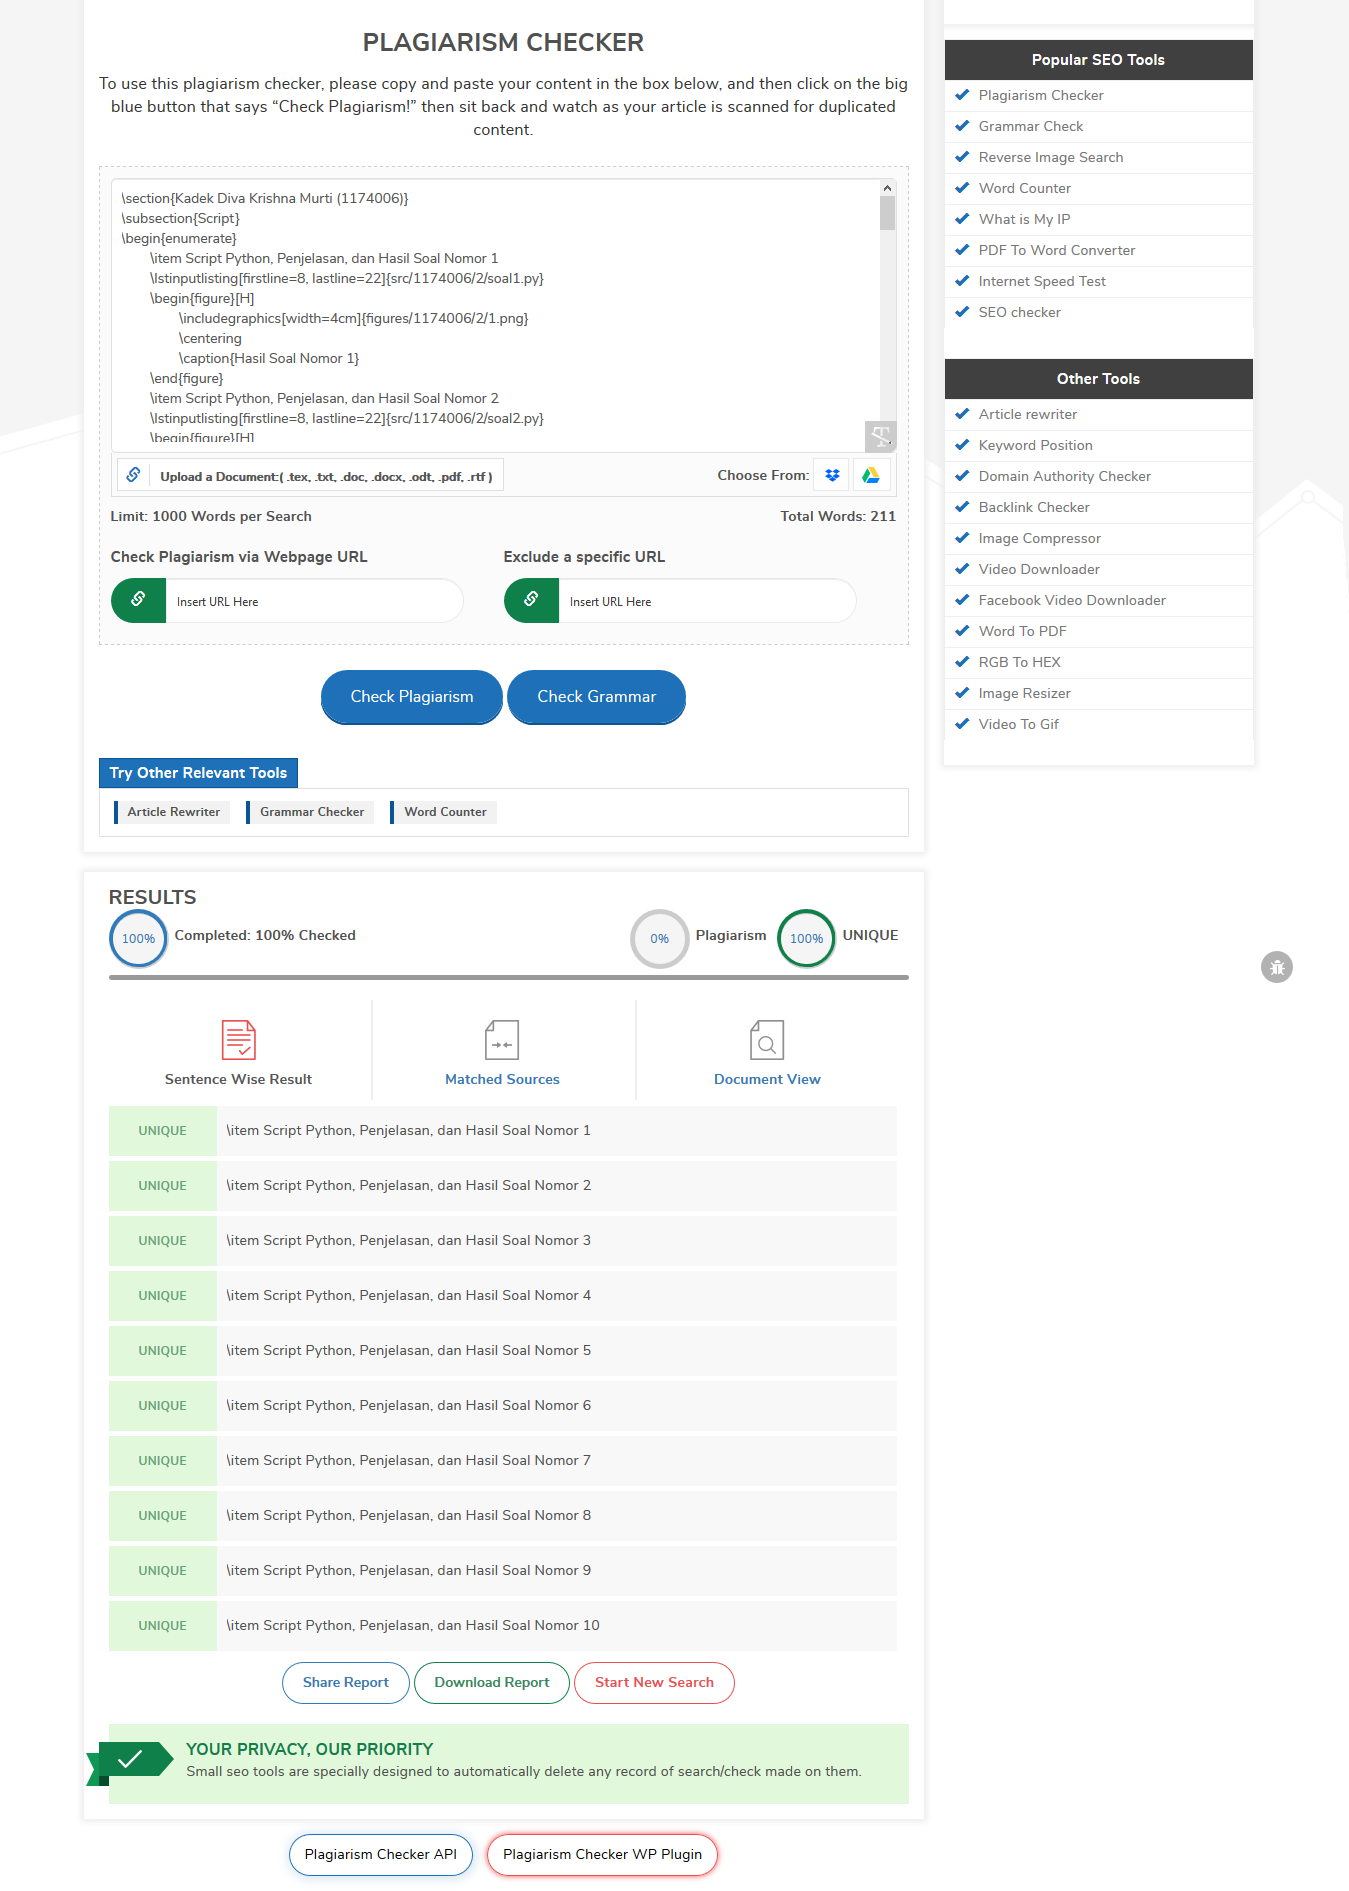
\includegraphics[width=4cm]{figures/1174006/2/plagiarism2.png}
	\centering
	\caption{Plagiarism Tugas 2 1174006}
\end{figure}